\chapter{Numerical Linear Algebra}
In this chapter we explore the primary questions of linear algebra: solving systems of
equations, approximating solutions to over-determined and under-determined systems of
equations, the eigenvalue-eigenvector problem, and the singular value problem. Along the
way we will encounter several novel ways to factor matrices into products of other
matrices with more desirable properties.


\section{Matrix Operations}
We start this chapter with the basics: the dot product and matrix multiplication.  MATLAB
is designed to do these tasks in very efficient ways but it is a good coding exercise to
build your own dot product and matrix multiplication routines.  You'll find in numerical
linear algebra that the indexing and the housekeeping in the codes is the hardest part, so
why don't we start easy.

\begin{problem}
    Recall that the dot product of two vectors $\bu, \bv \in \mathbb{R}^n$ is 
    \[ \bu \cdot \bv = \sum_{j=1}^n u_j v_j. \]
    Write a MATLAB function that accepts two vectors and returns the dot product. \\
    \mcode{function DotProduct = MyDotProduct(u, v)} \\
    It would be wise to put an error check in your code to make sure that the vectors are
    the same size.  You should be able to write this code without any loops.
\end{problem}

\begin{problem}
    Write a test script for the dot product of two random $n \times 1$ vectors.  Your
    script should output the absolute error between your dot product code and MATLAB's
    \mcode{dot}
    command.
\end{problem}

\begin{problem}
    Recall that if $A \in \mathbb{R}^{n \times p}$ and $B \in \mathbb{R}^{p \times m}$
    then the product $AB$ is defined as
    \[ \left( AB \right)_{ij} = \sum_{k=1}^p A_{ik} B_{kj}. \]
    A moments reflection reveals that each entry in the matrix product is actually a dot
    product, 
    \[ \left( AB \right)_{ij} = \left( \text{Row $i$ of matrix $A$} \right) \cdot \left(
    \text{Column $j$ of matirx $B$} \right). \]
    Write a MATLAB function that accepts two matrices and returns the matrix product. \\
    \mcode{function MatrixProduct = MatrixMultiply(A, B)} \\
    You
    should be able to write this code with only two loops; one for $i$ and one for $j$.
    The rest of the work should be done using dot products.
\end{problem}
\begin{problem}
    Write a test script for the matrix product of two random matrices of appropriate sizes.  Your
    script should output the normed error between your matrix product code and MATLAB's
    matrix multiplication.
\end{problem}



\section{Solving Systems of Linear Equations}
One of the many classic problems of linear algebra is to solve the linear system $A \bx =
\bb$. In this chapter we will spend a few days talking about efficient ways to have the computer solve
these systems. You likely recall row reduction (RREF) from previous linear algebra
courses, but the algorithm that you used is actually slow an cumbersome for computer
implementation.  Even so, let's blow the dust off of what you recall with a small practice
problem.

\begin{problem}
    Solve the following problem by hand using Gaussian Elimination (row reduction):
    \[ \begin{pmatrix} 1 & 2 & 3 \\ 4 & 5 & 6 \\ 7 & 8 & 0 \end{pmatrix} \begin{pmatrix}
            x_1 \\ x_2 \\ x_3 \end{pmatrix} = \begin{pmatrix} 1 \\ 0 \\ 2\end{pmatrix} \]
\end{problem}


\subsection{Upper and Lower Triangular Systems}
Row reduction works well on dense (or nearly dense) matrices but if the coefficient matrix
has special structure then we can avoid row reduction in lieu of faster algorithms. In the
following two problems you will devise algorithms for triangular matrices.

\begin{problem}
    Outline a fast algorithm (without formal row reduction) for solving the lower triangular system
    \[ \begin{pmatrix} 1 & 0 & 0 \\ 4 & 1 & 0 \\ 7 & 2 & 1 \end{pmatrix} \begin{pmatrix}
        y_1 \\ y_2 \\ y_3 \end{pmatrix} = \begin{pmatrix} 1 \\ 0 \\ 2\end{pmatrix}. \]
    As a convention we will always write our lower triangular matrices with ones on the
    main diagonal.  Your outline should be a list of explicit steps to solve the system.
    The most natural algorithm that most people devise here is called {\it forward
    substitution}.
\end{problem}


\begin{technique}[Forward Substitution: \texttt{LSolve}]\label{tech:lsolve}
    The following code solves the problem $L {\bf y} = \bb$ using forward
    substitution.  The matrix $L$ is assumed the be lower triangular with ones on the main
    diagonal.
\begin{lstlisting}
function y = LSolve(L , b)
n = length(b);
y = zeros(n,1);
for i = 1:n
    y(i) = b(i);
    for j = 1 : (i-1)
        y(i) = y(i) - L(i,j) * y(j);
    end
end
\end{lstlisting}
\end{technique}

\begin{problem}
    Consider the lower triangular system 
    \[ \begin{pmatrix} 1 & 0 & 0 \\ 4 & 1 & 0 \\ 7 & 2 & 1 \end{pmatrix} \begin{pmatrix}
        y_1 \\ y_2 \\ y_3 \end{pmatrix} = \begin{pmatrix} 1 \\ 0 \\ 2\end{pmatrix}. \]
    Work the code from Technique \ref{tech:lsolve} \underline{by hand} to solve the
    system.  Keep track of all of the indices as you work through the code.
\end{problem}

\begin{problem}
    Copy the code from Technique \ref{tech:lsolve} into a MATLAB function but in your code
    write a comment on every line stating what it is doing.  Write a test script that
    creates a lower triangular matrix of the correct form and a right-hand side $\bb$ and
    solve for ${\bf y}$.  Your code needs to work on systems of arbitrarily large size.
\end{problem}

\begin{problem}
    Outline a fast algorithm (without formal row reduction) for solving the upper triangular system
    \[ \begin{pmatrix} 1 & 2 & 3 \\ 0 & -3 & -6 \\ 0 & 0 & -9 \end{pmatrix}
        \begin{pmatrix} x_1 \\ x_2 \\ x_3 \end{pmatrix} = \begin{pmatrix} 1 \\ -4 \\
        3\end{pmatrix} \]
    The most natural algorithm that most people devise here is called {\it backward
    substitution}.
\end{problem}

\begin{technique}[Backward Substitution: \texttt{USolve}]\label{tech:usolve}
    The following code solves the problem $U {\bf x} = {\bf y}$ using backward
    substitution.  The matrix $U$ is assumed the be upper triangular.  You'll notice that
    most of this code is incomplete.  It is your job to complete this code.
\begin{lstlisting}
function x = USolve(U , y)
n = length(y);
x = zeros(n,1);
for i = ? : ? : ?        % what should you be looping over?
    x(i) = y(i) / ???;   % what should you be dividing by?
    for j = ? : ? : ?    % what should you be looping over? 
        x(i) = x(i) - U(i,j) * x(j) / ???;  % what should you be dividing by?
    end
end
\end{lstlisting}
\end{technique}

\begin{problem}
    Consider the upper triangular system
    \[ \begin{pmatrix} 1 & 2 & 3 \\ 0 & -3 & -6 \\ 0 & 0 & -9 \end{pmatrix}
        \begin{pmatrix} x_1 \\ x_2 \\ x_3 \end{pmatrix} = \begin{pmatrix} 1 \\ -4 \\
        3\end{pmatrix} \]
    Work the code from Technique \ref{tech:usolve} \underline{by hand} to solve the
    system.  Keep track of all of the indices as you work through the code.
\end{problem}

\begin{problem}
    Copy the code from Technique \ref{tech:usolve} into a MATLAB function but in your code
    write a comment on every line stating what it is doing.  Write a test script that
    creates an upper triangular matrix of the correct form and a right-hand side ${\bf y}$ and
    solve for ${\bf x}$.  Your code needs to work on systems of arbitrarily large size.
\end{problem}

\subsection{The LU Factorization}
\begin{problem}
    Open a new MATLAB script and enter the left-hand matrix of the previous problem into
    matrix $A$.  Observe what happens when we do the following in sequence:
    \begin{itemize}
        \item left multiply $A$ by the matrix
            \[ L_1 = \begin{pmatrix} 1 & 0 & 0 \\ -4 & 1 & 0 \\ 0 & 0 & 1 \end{pmatrix} \]
            This gives the matrix $L_1 A$.
        \item left multiply $L_1 A$ by the matrix
            \[ L_2 = \begin{pmatrix} 1 & 0 & 0 \\ 0 & 1 & 0 \\ -7 & 0 & 1 \end{pmatrix} \]
            This gives the matrix $L_2 L_1 A$.
        \item left multiply $L_2 L_1 A$ by the matrix 
            \[ L_3 = \begin{pmatrix} 1 & 0 & 0 \\ 0 & 1 & 0 \\ 0 & -2 & 1 \end{pmatrix} \]

    \end{itemize}
    Make a conjecture: If you wanted to multiply row $j$ of an $n\times n$ matrix by $c$
    and add it to row $k$, that is the same as multiplying by what lower triangular
    matrix?
\end{problem}

\begin{problem}
    After the process from the previous problem you should notice that you now have an
    upper triangular matrix.  Hence, in general, we have done this:
    \[ L_3 L_2 L_1 A = U, \]
    so if you solve for $A$ we see that $A$ can be written as
    \[ A = L_1^{-1} L_2^{-1} L_3^{-1} U. \]
    
    Therefore, we could rewrite the problem $A \bx = \bb$ as the
    problem $LU\bx = \bb$ where $L$ is which matrix?
\end{problem}
\solution{
    $L = L_1^{-1} L_2^{-1} L_3^{-1}$
}


\begin{problem}
    In the previous problem you likely found that $L = L_1^{-1} L_2^{-1} L_3^{-1}$.  Use
    MATLAB to find $L_j^{-1}$ for each $j$ and discuss general observations about how to
    find inverses of lower triangular matrices.  
\end{problem}

\begin{problem}
    Now for the punch line: If we can write $A \bx = \bb$ then if we can write it as $LU
    \bx = \bb$ we can
    \begin{enumerate}
        \item Solve $L \by = \bb$ for $\by$ using forward substitution.  Then,
        \item solve $U \bx = \by$ for $\bx$ using backward substitution.
    \end{enumerate}
    For our running example, write down $L$ and $U$ and solve the system.
\end{problem}

\begin{problem}
    Try the process again on the $3\times 3$ system of equations
    \[ \begin{pmatrix}
        3 & 6 & 8\\
        2 & 7 & -1 \\
        5 & 2 & 2 
    \end{pmatrix} \begin{pmatrix} x_1 \\ x_2 \\ x_3 \end{pmatrix} = 
        \begin{pmatrix} -13 \\ 4 \\ 1 \end{pmatrix} \]
    That is: Find matrices $L$ and $U$ such that $A \bx = \bb$ can be written as $LU\bx =
    \bb$.  The do two triangular solves to determine $\bx$.\\
    Notice that this time there isn't a ``$1$'' in the top left corner to begin with.  Be
    careful.
\end{problem}


\begin{technique}[LU Factorization]\label{tech:lu}
    The following MATLAB function takes a square matrix $A$ and
    outputs the matrices $L$ and $U$ such that $A = LU$.  Partial code is given below.
    Complete the code.
\begin{lstlisting}
function [L,U] = MyLU(A)
n = size(A,1);      % finds the size of the matrix
if size(A,1) ~= size(A,2)   % what does this do?
    fprintf('Error: The matrix A is not square\n')
    break
end
L = eye(n,n);       % initialize L as an identity matrix (why?)
U = A;              % initialize U as A (why?)
for j = 1 : (n-1)   % loop over the columns
    for i = (j+1) : n   % loop over the rows
        mult = A(i,j) / A(j,j); % what does this line do?
        A(i, j+1:n) = A(i, j+1:n) - mult*A(j, j+1:n);
        U(i, j+1:n) = ???   % what part of A should you be putting in U here?
        L(i,j) = ???        % what should go in the lower triangular matrix?
        U(i,j) = 0;         % zero out the bottom portion of U (why?)
    end
end
\end{lstlisting}
\end{technique}

\begin{thm}[LU Factorization Algorithm]
    Let $A$ be a square matrix in $\mathbb{R}^{n \times n}$ and let $\bx, \bb \in
    \mathbb{R}^n$.  To solve the problem $A \bx =\bb$,
    \begin{enumerate}
        \item Factor $A$ into lower and upper triangular matrices $A = LU$.\\
            \mcode{[L, U] = MyLU(A);}
        \item The system can now be written as $LU \bx = \bb$.  Substitute $U \bx = {\bf
            y}$ and solve the system $L {\bf y} = \bb$ with forward substitution. \\
            \mcode{y = LSolve(L, b);}
        \item Finally, solve the system $U \bx = {\bf y}$ with backward substitution. \\
            \mcode{x = USolve(U, y);}
    \end{enumerate}
\end{thm}

\begin{problem}
    Test your \mcode{MyLU}, \mcode{LSolve}, and \mcode{USolve} functions on a linear
    system for which you know the answer.  Then test your problem on a system
    that you don't know the solution to.  Discuss where your code will fail. Use the
    following partial code to test your functions.
\begin{lstlisting}
A = [...; ...; ... ];
b=  [...; ...; ... ];
[L,U] = MyLU(A);
y = Lsolve(L,b);
x = Usolve(U,y)
MATLABExactAnswer = A\b
MyError = norm(x-MATLABExactAnswer)
\end{lstlisting}
\end{problem}


% \begin{problem}
%     {\bf Coding Challenge:} In the $20\times20$ grid below, four numbers along a diagonal line
%     have been marked in red.
%     \begin{center}
%         \begin{tabular}{cccccccccccccccccccc}
%     08&02&22&97&38&15&00&40&00&75&04&05&07&78&52&12&50&77&91&08\\
%     49&49&99&40&17&81&18&57&60&87&17&40&98&43&69&48&04&56&62&00\\
%     81&49&31&73&55&79&14&29&93&71&40&67&53&88&30&03&49&13&36&65\\
%     52&70&95&23&04&60&11&42&69&24&68&56&01&32&56&71&37&02&36&91\\
%     22&31&16&71&51&67&63&89&41&92&36&54&22&40&40&28&66&33&13&80\\
%     24&47&32&60&99&03&45&02&44&75&33&53&78&36&84&20&35&17&12&50\\
%     32&98&81&28&64&23&67&10&{\color{red} {\bf 26}}&38&40&67&59&54&70&66&18&38&64&70\\
%     67&26&20&68&02&62&12&20&95&{\color{red} {\bf 63}}&94&39&63&08&40&91&66&49&94&21\\
%     24&55&58&05&66&73&99&26&97&17&{\color{red} {\bf 78}}&78&96&83&14&88&34&89&63&72\\
%     21&36&23&09&75&00&76&44&20&45&35&{\color{red} {\bf 14}}&00&61&33&97&34&31&33&95\\
%     78&17&53&28&22&75&31&67&15&94&03&80&04&62&16&14&09&53&56&92\\
%     16&39&05&42&96&35&31&47&55&58&88&24&00&17&54&24&36&29&85&57\\
%     86&56&00&48&35&71&89&07&05&44&44&37&44&60&21&58&51&54&17&58\\
%     19&80&81&68&05&94&47&69&28&73&92&13&86&52&17&77&04&89&55&40\\
%     04&52&08&83&97&35&99&16&07&97&57&32&16&26&26&79&33&27&98&66\\
%     88&36&68&87&57&62&20&72&03&46&33&67&46&55&12&32&63&93&53&69\\
%     04&42&16&73&38&25&39&11&24&94&72&18&08&46&29&32&40&62&76&36\\
%     20&69&36&41&72&30&23&88&34&62&99&69&82&67&59&85&74&04&36&16\\
%     20&73&35&29&78&31&90&01&74&31&49&71&48&86&81&16&23&57&05&54\\
%     01&70&54&71&83&51&54&69&16&92&33&48&61&43&52&01&89&19&67&48
% \end{tabular}
% \end{center}
% 
%     The product of these numbers is $26 \times 63 \times 78 \times 14 = 1788696$.  Write
%     code to find the greatest product of four adjacent numbers in the same direction (up, down,
%     left, right, diagonally (down and right), or diagonally (down and left)) in the $20\times20$ grid?
% \end{problem}
% % \solution{Source: Project Euler Problem \#11: Solution: 70600674 }


\begin{problem}
    For this problem we are going to run a numerical experiment to see how the process of
    solving the equation $A \bx = \bb$ using the $LU$ factorization performs.\\ 
    \noindent Create a loop that does the following
    \begin{itemize}
        \item Build a random matrix of size $n \times n$. You can do this with the code:
            \\
            \mcode{A=rand(n,n)}
        \item Build a random vector in $\mathbb{R}^{n}$. You can do this with the code: \\
            \mcode{b = rand(n,1)}
        \item Find MATLAB's exact answer to the problem $A\bx=\bb$ using the backslash: \\
            \mcode{Xexact = A\b}
        \item Write code that uses your three $LU$ functions (\mcode{MyLU, Lsolve,
            Usolve}) to find a solution to the equation $A\bx=\bb$.
        \item Find the error between your answer and the exact answer using the code: \\
            \mcode{error = norm(x - Xexact)}
        \item Make a plot that shows how the error behaves as the size of the problem
            changes. You should run this for matrices of larger and larger size but be
            warned that the loop will run for quite a long time if you go above
            $300×300$ matrices. Just be patient.
    \end{itemize}
\end{problem}

\section{The Least Squares Problems}
\begin{problem}\label{prob:least_squares_1}
    Download the Excel data set from Moodle.  We're going to develop a way to match the
    data sets using linear algebra.  Before doing the linear algebra versions of this
    problem though we'll use Excel to match the data sets.  Our goal is to make a guess at
    the type of polynomial that models the function (given in this case) and to minimize
    the error between our guess and the data.  Follow these steps in Excel to find best
    fitting curves.  We'll start with the linear data.
    \begin{enumerate}
        \item In column C set up a function for your guess of the model based on the $x$ data in column
            $A$.  You will need to set up cells for the polynomial parameters (for the
            linear case these are the slope and the $y$-intercept).
        \item Fill in your guesses based on initial approximations for the slope and
            $y$-intercept.
        \item Use column D to calculate the residual value for each data point.
            \[ \text{Residual} = \text{Actual $y$ Value - Approximate $y$ Value} \]
        \item Use column E to calculate the square of the residual for each data point.
        \item Our goal is the minimize the sum of the squares of the residuals.
            \[ \text{min} \left( \sum_{j=1}^n \left( y_j - \hat{y}_j \right)^2 \right) \]
            For this we can use the \texttt{Excel Solver} to minimize the sum of the
            square residuals.
    \end{enumerate}
    Now repeat the process for the quadratic and cubic data.
\end{problem}




At this point we need to discuss the quality of the fits that we are building.  You are
likely familiar with the $R$ and $R^2$ values from statistics, but let's just recap here.  
\begin{definition}[Correlation Coefficient, $R$]
    The {\bf correlation coefficient}, $R$, is a measure of the quality of a linear fit.
    \begin{itemize}
        \item If $R = +1$ then the data represent a perfect linear fit with a positive slope. 
        \item If $R = -1$ then the data represent a perfect linear fit with a negative
            slope.  
        \item If $R = 0$ then there is no linear relationship between the two variables.
    \end{itemize}
\end{definition}

\begin{definition}[Coefficient of Determination, $R^2$]
    The {\bf coefficient of determination}, $R^2$, is the proportion of variance in the
    dependent ($y$) variable that is explained by the independent ($x$) variable.  
    \begin{itemize}
        \item If $R^2 = 1$ then 100\% of the variance in $y$ is explained by $x$ and the
            fit is perfect. 
        \item If $R^2 = 0$ then 0\% of the variance in $y$ is explain by $x$ and there is
            no correlation between the two variables.
    \end{itemize}
\end{definition}

In the problems that we've studied thus far we have calculated the sum of the squares of
the residuals as a measure of how well our function fits the data.  The trouble with the
sum of the squares of the residuals is that it is context dependent.  Hence, there is no
way to tell at the outset what a {\it good} sum of squares of residuals is.  

\begin{thm}
    To calculate the $R^2$ value we can use the following equations where $y_j$ is the
    $j^{th}$ data point, $\bar{y}$ is the mean $y$-value in the data, and $f_j$ is the
    $j^{th}$ predicted output from our model.
    \begin{flalign}
        \text{Total Sum of Squares: } & TSS = \sum_j \left( y_j - \bar{y} \right)^2
        \label{eqn:TSS} \\
        \text{Residual Sum of Squares: } & RSS = \sum_j \left( y_j - f_j \right)^2 
        \label{eqn:RSS} \\
        \text{Coeff. of Determination: } & R^2 = 1 - \frac{RSS}{TSS} \label{eqn:Rsquared}
    \end{flalign}
\end{thm}

\begin{problem}
    Compute the $R^2$ value for each of the data sets from Problem
    \ref{prob:least_squares_1}.
\end{problem}

\begin{problem}
    Use equation \eqref{eqn:Rsquared} to explain why $R^2=1$ implies a perfect fit.
\end{problem}
\solution{
    If $R^2 = 1$ then $RSS = 0$ and this implies that there are no residuals.  Hence we
    have made no errors with our model.
}

There are MANY statistics packages out there that will do least squares regression for us.
MATLAB has the \texttt{polyfit} command, R has the \texttt{lm} command, and Excel has the
data analysis toolpack.  Behind the scenes in all of these is actually linear algebra.  It
is informative pedagogically to do the least squares problems using Excel a few times (as
we did in Problem \ref{prob:least_squares_1}), but in reality there is some beautifully
simple linear algebra behind the scenes.

\begin{problem}
    Now we'll use Linear Algebra to complete the same types of problems.  Set up a
    \texttt{MATLAB} script the reads the linear data from the Excel sheet.  We are
    assuming that the data are linear so for each $x$-value $x_j$ we assume that the equation 
    \[ c_0 + c_1 x_j \approx y_j. \]
    This gives rise to a system of linear equations
    \[ \begin{pmatrix} 1 & x_1 \\ 1 & x_2 \\ 1 & x_3 \\ \vdots & \vdots \\ 1 & x_n
        \end{pmatrix} \begin{pmatrix} c_0 \\ c_1 \end{pmatrix} \approx \begin{pmatrix} y_1
            \\ y_2 \\ y_3 \\ \vdots \\ y_n \end{pmatrix} \]
    We'll call the left-hand matrix $A$ and the right-hand vector $\by$.  
    \begin{enumerate}
        \item Get $A$ and $\by$ into \texttt{MATLAB} so we can use them.
        \item This is not a square system. In fact, it is {\it overdetermined}.  Consider
            that the column space of $A$ ($Col(A)$) is a subspace of $\mathbb{R}^n$ and
            that $\by \in \mathbb{R}^n$ is likely not in the column space of $A$.  If we
            project $\by$ onto $Col(A)$ we should be able to find the best approximation
            of $\by$ that lies in $Col(A)$. 

            Projections onto a subspace can be achieved with matrix multiplication, but
            which matrix shall we multiply by \dots

            \[ (??) A \begin{pmatrix} c_0 \\ c_1 \end{pmatrix}  = (??) \by. \]

            Once you are satisfied that the right-hand side is a projection of $\by$ onto
            $Col(A)$ you have formed the {\bf normal equations}.  If you've done everthing
            right then you also now have a square system ($2 \times 2$ in this case).

        \item Now that this is a square matrix you can solve for $c_0$ and $c_1$ using
            your $LU$ code. (You can also use \texttt{MATLAB}'s {\it backslash} (\verb|\|) command to
            do the linear solve)
        \item Now that you have $c_0$ and $c_1$ you can form the linear approximation.
            Plot the approximation along with your data.  Also write code to plot the
            residuals (subplot would be great here).
        \item Repeat the process for the quadratic and cubic data.  For the quadratic data
            you are assuming that 
            \[ c_0 + c_1 x_j + c_2 x_j^2 \approx y_j, \]
            and for the cubic data you are assuming that 
            \[ c_0 + c_1 x_j + c_2 x_j^2 + c_3 y_j^3 \approx y_j. \]
    \end{enumerate}
\end{problem}


\begin{definition}[The Normal Equations]
    Let $A \in \mathbb{R}^{n \times m}$, ${\bf c} \in \mathbb{R}^{m}$, and $\by \in
    \mathbb{R}^n$ where $n \gg m$.  The system of equations
    \[ A {\bf c} = \by \]
    is over determine since there are more equations than unknowns.  Multiply both sides
    of the equation by $A^T$ yields the {\bf normal equations}
    \[ A^T A {\bf c} = A^T \by. \]
    We note here that $A^T A \in \mathbb{R}^{m \times m}$ is square and much smaller than
    $A$.  The right-hand side of the normal equations is the projection of $\by$ onto the
    columns space of $A$.  
\end{definition}

\begin{problem}
    In the same Excel document you will find a set of data representing a nonlinear
    function.  Use Excel to find the best fit curve by making a {\it guess} about the form
    of the function.  Since this is a nonlinear relationship our method of using the
    normal equations will not work.
\end{problem}

\begin{problem}
    The method of using the {\bf normal equations} to solve a least squares regression
    problem also works for multiple regression.  In this example go to the second tab of
    the Excel document to find the Hollywood Box Office Receipts (measured in millions).
    We are seeking a model of the form
    \[ X_1  \approx \beta_1 + \beta_2 X_2 + \beta_3 X_3. \]
    That is, we seek to predict first year box office receipts ($X_1$) from production
    cost data ($X_2$) and promotional cost data ($X_3$).
    \begin{itemize}
        \item Read the data into MATLAB
        \item Find the matrix $A$ to form the overdetermined system of equations
            \[ A \begin{pmatrix} \beta_1 \\ \beta_2 \\ \beta_3 \end{pmatrix} =
                    \bx_1 \]
        \item Form the normal equations and solve for $\beta_1, \beta_2,$ and $\beta_3$.  
        \item Star Wars: The Force Awakens had a production cost of \$32M and a
            promotional cost of only \$17M.  What does our model predict about the first
            year box office receipts?
    \end{itemize}
\end{problem}

% 
% \begin{problem}
%     Let's go back to the World Health Organization, but this time you're looking for a
%     data set where you can use \underline{multiple regression} (linear or polynomial).
%     Give a full description of the data set, discuss why regression is a sensible thing to
%     do, find a regression model, and make a prediction using your regression model.
% \end{problem}
% 


\section{The QR Factorization}
Our goal in this section is to improve the efficiency of solving the least squares
problems via the normal equations.  Recall that we want to find $\bx$ such that $A \bx =
\bb$ but where $\bb$ is not in the column space of $A$.  This necessitated the use of the
normal equations $A^T A \bx = A^T \bb$ to project $\bb$ onto the column space of $A$.
This would be FAR more efficient if the columns of $A$ were orthogonal (perpendicular) and
normalized (unit vectors).  Hence, our goal is to take $A$ and factor it into $A = QR$
where the columns of $Q$ are orthonormal (orthogonal and normalized) and $R$ is an upper
triangular matrix.

\begin{problem}
    First we'll do a problem by hand: \\
    Consider the matrix $A = \begin{pmatrix} 1 & 1 & 0 \\ 1 & 0 & 1 \\ 0 & 1 & 1
    \end{pmatrix}$.  We want to factor $A$ into $A = QR$ where the columns of $Q$ are
    orthonormal and $R$ is upper triangular.  Here is the algorithm (run every step by
    hand!).  For notation purposes, $\ba_j$ will be the $j^{th}$ column of $A$.
    \begin{enumerate}
        \item Define $\bq_1 = \displaystyle \frac{\ba_1}{\|\ba_1\|}$.  This will be the
            first column of $Q$.\\
%             \teacher{
%                 \[ \bq_1 = \begin{pmatrix} 1/\sqrt{2} \\ 1/\sqrt{2} \\ 0 \end{pmatrix} \]
%             }
        \item Define $\bq_2 = \displaystyle \ba_2 - \left( \ba_2 \cdot \bq_1 \right)
            \bq_1$.  Once you've done this calculation normalize your result so
            $\displaystyle \bq_2 = \frac{\bq_2}{\|\bq_2\|}$. This is the second column
            of $Q$.  \\Explain the geometry of this step (DRAW A PICTURE!)\\
%             \teacher{
%                 \[ \bq_2 = \begin{pmatrix} 1\\0\\1\end{pmatrix} - \frac{1}{\sqrt{2}}
%                         \begin{pmatrix} 1/\sqrt{2} \\ 1/\sqrt{2} \\0\end{pmatrix} =
%                             \begin{pmatrix} 1/2 \\ -1/2 \\ 1 \end{pmatrix} \quad \bu_2 =
%                                 \begin{pmatrix} 1/\sqrt{6} \\ -1/\sqrt{6} \\ 2/\sqrt{6}
%                                 \end{pmatrix} \]
%             }
        \item Define $\bq_3 = \displaystyle \ba_3 - \left( \ba_3 \cdot \bq_1 \right)\bq_1
            - \left( \ba_3 \cdot \bq_2 \right)\bq_2$ and then redefine $\displaystyle
            \bq_3 = \frac{\bq_3}{\|\bq_3\|}$.  This is now the third column of
            $Q$.\\
%             \teacher{
%             \[ \bq_3 = \begin{pmatrix} -1/\sqrt{3} \\ 1/\sqrt{3} \\ 1/\sqrt{3}
%                 \end{pmatrix} \]
%             }
        \item The matrix $R$ is formed as follows:
            \[ R = \begin{pmatrix} \ba_1 \cdot \bq_1 & \ba_2 \cdot \bq_1 & \ba_3 \cdot
                    \bq_1 \\ 0 & \ba_2 \cdot \bq_2 & \ba_3 \cdot \bq_2 \\ 0 & 0 & \ba_3
                    \cdot \bq_3 \end{pmatrix} \]
%             \teacher{
%             \[ R = \begin{pmatrix} 2/\sqrt{2} & 1/\sqrt{2} & 1/\sqrt{2} \\ 0 & 3/\sqrt{6}
%                     & 1\/\sqrt{6} \\ 0 & 0 & 2/\sqrt{3} \end{pmatrix} \]
%             }
        \item Write down $Q$ and observe that the process is just begging for several
            loops on a computer to implement this on bigger matrices.
        \item Use MATLAB to check that $A = QR$.
        \item Finally let's look at the utility of the result:
            \begin{enumerate}
                \item Since $Q$ is an orthonormal matrix $Q^TQ$ is the identity matrix!
                    (Explain why.)
                \item If we want to solve $A\bx = \bb$ and we can write $A = QR$ then 
                    \[ A \bx = \bb \quad \implies \quad QR \bx = \bb \quad \implies \quad
                        R \bx = Q^T \bb \]
                \item Since $R$ is upper triangular we can use the \mcode{Usolve} code we
                    have from our work with the LU-factorization to solve for $\bx$.  THIS
                    IS REALLY FAST!!
                \item Compare this to the number of computer operations needed so solve
                    the normal equations $A^TA\bx = A^T \bb$ with an $LU$-solver.
            \end{enumerate}
    \end{enumerate}
\end{problem}

\begin{problem}
    Write MATLAB code that takes a matrix $A$ (not necessarily square) and outputs the
    both the $Q$ matrix and the $R$ matrix. Pseducode for this function is as follows:
    \begin{itemize}
        \item Set up the function call:\\ \mcode{function [Q,R] = MyQR(A)}
        \item Set up \mcode{zeros} matrices for both $Q$ and $R$.  Remember that $A$ may
            not be square so assume that the columns are in $\mathbb{R}^m$ and the rows
            are in $\mathbb{R}^n$.  Hence $Q$ will be $m \times n$ and $R$ will be $n
            \times n$.
        \item Start a loop that counts across the columns:\\ \mcode{for j=1:n}
            \begin{itemize}
                \item define a temporary variable: $\hat{\bq} = \ba_j$
                \item start a loop that will do all of the subtractions and build some of
                    the $R's$:\\ \mcode{for i=1:j-1}
                    \begin{itemize}
                        \item build one of the $R's$: $R_{ij} = \ba_j \cdot \bq_i$
                        \item Do one of the subtractions: $\hat{\bq} = \hat{\bq} - R_{ij} \bq_i$
                    \end{itemize}
                \item end the loop for \mcode{i}
                \item normalize the $j^{th}$ column in $Q$: $\bq_j = \hat{\bq} / \| \hat{\bq} \|$
                \item build the $R's$ on the diagonal: $R_{jj} = \ba_j \cdot \bq_j$
            \end{itemize}
        \item end the loop for \mcode{j}
    \end{itemize}
\end{problem}

\begin{problem}
    Write a script that tests your \mcode{MyQR} function on randomly generated $m×n$ matrices
    with randomly generated right-hand sides. Compare the time that it takes to solve the
    least squares problems using QR to the time necessary to solve with LU via the normal
    equations. When is LU more efficient? When is QR more efficient?
\end{problem}

\begin{problem}
    Now that you have $QR$ and $LU$ code we're going to use both of them!  The problem is
    as follows: \\
    We are going to find the polynomial of degree 4 that best fits the function $y =
    \cos(4t) + 0.1 \varepsilon(t)$ at 50 equally spaced points $t$ between $0$ and $1$.  Here
    we are using $\varepsilon(t)$ as a function that outputs normally distrubuted random
    white noise.  In \texttt{MATLAB} you will build $y$ as \\
    \mcode{y = cos(4*t) + 0.1*randn(size(t));}
    
    Build the $t$ vector
    and the $y$ vector (these are your data).  We need to set up the least squares
    problems $A \bx = \bb$ by setting up the matrix $A$
    as we did in the other least squares curve fitting problems and by setting up the
    $\bb$ vector using the $y$ data you just built.  
    \begin{enumerate}
        \item[(a)] Solve the normal equations $A^T A \bx = A^T \bb$ using your $LU$ code.
        \item[(b)] Solve the system $A \bx = \bb$ by first transforming $A$ to $A = QR$
            and then solving $R\bx = Q^T \bb$.
        \item[(c)] Use \texttt{MATLAB} to find the sum of the square errors between the
            polynomial approximation and the function $f(t) = \cos(4t)$ for both the $QR$
            and the $LU$ approaches.  
        \item[(d)] Build \texttt{MATLAB} code that does parts (a) - (c) several hundered
            times and complies results comparing which method gives the better
            approximation (smaller sum of square error).
    \end{enumerate}
\end{problem}


\section{The Eigenvalue-Eigenvector Problem}
Recall that the eigenvectors, $\bx$, and the eigenvalues, $\lambda$ of a square matrix satisfy the
equation $A\bx=\lambda \bx$. Geometrically, the eign-problem is the task of finding the special
vectors $\bx$ such that multiplication by the matrix $A$ only produces a scalar multiple of
$\bx$. Thinking about matrix multiplication, this is rather peculiar since matrix-vector
multiplication usually results in a scaling and a rotation of the vector. Therefore, in
some sense the eigenvectors are the only special vectors which avoid geometric rotation
under matrix multiplication.  For a graphical exploration of this idea see:
\href{https://www.geogebra.org/m/JP2XZpzV}{https://www.geogebra.org/m/JP2XZpzV}.

Recall that to solve the eigen-problem for a square matrix $A$ we complete the following
steps:
\begin{enumerate}
    \item First rearrange the definition of the eigenvalue-eigenvector pair to 
        \[ (A\bx−\lambda \bx)=\bo. \]
    \item Next, factor the $\bx$ on the right to get 
        \[ (A−\lambda I) \bx=\bo. \]
    \item Now observe that since $\bx \ne 0$ the matrix $A−\lambda I$ must NOT have an inverse. Therefore,
        \[ \det(A−\lambda I)=0. \]
    \item Solve the equation $\det(A−\lambda I)=0$ for all of the values of $\lambda$.
    \item For each $\lambda$, find a solution to the equation $(A−\lambda I) \bx=\bo$.
        Note that there will be infinitely many solutions so you will need to make wise
        choices for the free variables.
\end{enumerate}
\begin{problem}
    Find the eigenvalues and eigenvectors of $A = \begin{pmatrix} 1 & 2 \\ 4 & 3
    \end{pmatrix}$ by hand.
\end{problem}
% \teacher{the eigenvalues of $\lambda_1 = -1$ and $\lambda_2 = 5$ with eigenvectors $\bv_1
%     = (1,-1)^T$ and $\bv_2 = (1,2)^T$
% }

\begin{problem}
    In the matrix $A = \begin{pmatrix} 1 & 2 & 3 \\ 4 & 5 & 6 \\ 7 & 8 & 9 \end{pmatrix}$
    one of the eigenvalues is $\lambda_1 = 0$.
    \begin{enumerate}
        \item What does that tell us about the matrix $A$?
%             \teacher{$A$ is not invertible. }
        \item What is the eigenvector $\bv_1$ associated with $\lambda_1 = 0$?
%             \teacher{$\bv_1 = (1,-2,1)^T$}
    \end{enumerate}
\end{problem}

\begin{problem}
    Find matrices $P$ and $D$ such that $A = \begin{pmatrix} 1 & 2 \\ 4 & 3 \end{pmatrix}$
        can be written as $A = PDP^{-1}$ where $P$ is a dense $2 \times 2$ matrix and $D$
        is a diagonal matrix.  Once you have this factorization of $A$, use it to
        determine $A^{10}$.
\end{problem}
% \teacher{
%     \[ P = \begin{pmatrix} 1 & 1 \\ -1 & 2 \end{pmatrix} \quad D = \begin{pmatrix} -1 & 0
%             \\ 0 & 5 \end{pmatrix} \quad P^{-1} = \begin{pmatrix} 2/3 & -1/3 \\ 1/3 & 1/3
%             \end{pmatrix} \]
%             \[ A^{10} = P D^{10} P^{-1} = P \begin{pmatrix} 1 & 0 \\ 0 & 9765625
%                 \end{pmatrix} P^{-1} \]
% }

\begin{problem}
    Let $A$ be an $n \times n$ matrix with $n$ distinct eigenvectors $\bv_1, \bv_2, \dots,
    \bv_n$ and let $\bx \in \mathbb{R}^n$ be a vector such that $\bx = \sum_{j=1}^n c_j
    \bv_j$. Find expressions for $A\bx$, $A^2 \bx$, $A^3\bx$, \dots
\end{problem}
% \teacher{
%     \[ A^k\bx = \sum_{j=1}^n c_j \lambda_j^k \bv_j \]
% }

\begin{problem}
    In this problem  we first describes the mathematical idea for the {\bf power method} for
    computing the largest eigenvalue / eigenvector pair.  Then we write an algorithm for
    find the largest eigen-pair numerically.
    \begin{enumerate}
        \item Assume that $A$ has $n$ linearly independent eigenvectors $\bv_1, \bv_2,
            \dots, \bv_n$ and choose $\bx =
            \sum_{j=1}^n c_j \bv_j$.  From the previous problem,
            \[ A^k \bx = \underline{\hspace{2in}} \]
% \teacher{
%     \[ A^k\bx = \sum_{j=1}^n c_j \lambda_j^k \bv_j \]
% }
        \item Factor the right-hand side so that 
            \[ A^k \bx = \lambda_1^k \left( c_1 \bv_1 + c_2 \left(
                \frac{\lambda_2}{\lambda_1} \right)^k \bv_2 + c_3 \left(
                \frac{\lambda_3}{\lambda_1}
                \right)^k \bv_3 + \cdots + c_n \left( \frac{\lambda_n}{\lambda_1}
                \right)^k \bv_n \right) \]
        \item If $\lambda_1 > \lambda_2 \ge \lambda_3 \ge \cdots \ge \lambda_n$ then what
            happens to each of the $(\lambda_j/\lambda_1)^k$ terms as $k \to \infty$?
            Using this answer, what is $\lim_{k \to \infty} A^k \bx$?\\
%             \teacher{
%                 \[ \lim_{k \to \infty} A^k \bx = \lambda_1^k c_1 \bv_1 \]
%             }
    \end{enumerate}

    {\bf The Power Method Algorithm:} This algorithm will quickly find the 
    eigenvalue of largest absolute value for a square matrix $A \in \mathbb{R}^{n \times
    n}$ as well as the associated (normalized) eigenvector.  We are
    assuming that there are $n$ linearly independent eigenvectors of $A$.
    \begin{description}
        \item[Step \#1:] Given a nonzero vector $\bx$, set $\bv^{(1)} = \bx / \|\bx\|$.
            (Here the superscript indiates the iteration number)
        \item[Step \#2:] For $k=2, 3, \ldots$
            \begin{description}
                \item[Step \#2a:] Compute $\tilde{\bv}^{(k)} = A \bv^{(k-1)}$ (this gives
                    a non-normalized version of the next estimate of the dominant
                    eigenvector.)
                \item[Step \#2b:] Set $\lambda^{(k)} = \left< \tilde{\bv}^{(k)} ,
                    \bv^{(k-1)} \right>$.  (this gives an approximation of the eigenvalue
                    since if $\bv^{(k-1)}$ was the actual eigenvector we would have
                    $\lambda = \left< A \bv^{(k-1)}, \bv^{(k-1)} \right>$)
                \item[Step \#2c:] Normalize $\tilde{\bv}^{(k)}$ by computing $\bv^{(k)} =
                    \tilde{\bv}^{(k)} / \| \tilde{\bv}^{(k)} \|$. (This guarantees that
                    you will be sending a unit vector into the next iteration of the loop)
            \end{description}
    \end{description}
\end{problem}

\begin{problem}
    Write a MATLAB function to implement the power method for finding the eigenvalue of
    largest absolute value and the associated eigenvector.  Test it on a matrix where you
    know the eigenvalue of interest.
\end{problem}


\section{The Singular Value Decomposition}
Our overarching goal of this section is to discuss an analogue to the
eigenvalue-eigenvector problem for non-square matrices.  That is, we would like to take a
matrix $A$ that is $m \times n$ and find vectors are values that behave similarly to how
eigenvectors and eigenvalues behave for square matrices.  The key to this discussion is
the matrix $A^T A$, so let's start there.

\begin{problem}
    Let $A$ be an $m \times n$ matrix.  What is the size of $A^T A$?  Prove that $A^T A$
    must be a symmetric matrix (a matrix $B$ is symmetric if $B_{ij} = B_{ji}$).  Finally, what bearing
    does the next Theorem have on the matrix $A^T A$?
\end{problem}
% \teacher{
%     Let $B = A^T A$.  Hence $B_{ij} = \ba_i \cdot \ba_j = \ba_j \cdot \ba_i = B_{ji}$.
%     Since $B$ is symmetric and real we know that $A^T A$ will have $n$ orthogonal
%     eigenvectors.
% }




\begin{thm}\label{thm:sym_matrix}
    An $n \times n$ matrix $A$ has $n$ orthogonal eigenvectors if and only if $A$ is a
    symmetric matrix.
\end{thm}


\begin{definition}
The {\bf singular values} of an $m \times n$ matrix $A$ are the square roots of $A^T A$.
They are typically denoted as $\sigma_1, \sigma_2, \dots, \sigma_n$ where $\sigma_j =
\sqrt{\lambda_j}$ and $\lambda_j$ is an eigenvalue of $A^T A$.  
\end{definition}

\begin{definition}
    The {\bf singular value decomposition} of an $m \times n$ matrix $A$ with rank $r$ is
    a factorization of $A$ into the product of three matrices, $U$, $\Sigma$, and $V$,
    such that
    \[ A = U \Sigma V^T. \]
    In the singular value decomposition, $U$ ($m \times m$) and $V$ ($n \times n$) have
    orthogonal columns and $\Sigma$ ($m \times n$)
    is a block diagonal matrix 
    \[ \Sigma = \begin{pmatrix} D & 0 \\ 0 & 0 \end{pmatrix} \]
    where $D$ is an $r \times r$ diagonal matrix containing the $r$ singular values of
    $A$ in rank order (largest to smallest).

    To build the singular value decomposition:
    \begin{enumerate}
        \item Form $A^TA$ and find the eigenvalues and eigenvectors (guaranteed to exist
            by Theorem \ref{thm:sym_matrix}).
        \item Form $\Sigma$
        \item The columns of $V$ are the eigenvectors of $A^T A$.
        \item The columns of $U$ are the normalized vectors obtained by 
            \[ \bu_1 = \frac{1}{\sigma_1} A \bv_1\, , \, \bu_2 = \frac{1}{\sigma_2} A
            \bv_2 \, , \, \dots, \, \bu_m = \frac{1}{\sigma_m} A \bv_m \]
    \end{enumerate}
\end{definition}

\begin{problem}
    Use MATLAB to find the singular value decomposition of 
    \[ A = \begin{pmatrix} 4 & 11 & 14 \\ 8 & 7 & -2 \end{pmatrix} \]
    Some practical MATLAB tips follow:
    \begin{enumerate}
        \item Define $A$
        \item Define the sizes: \mcode{m=size(A,1); n=size(A,2)}
        \item Find the rank of $A$: \mcode{r = rank(A);}
        \item Define the matrices \mcode{Sigma} and \mcode{U} to be zero matrices with
            the right size.
        \item Have MATLAB calculate the eigenvectors and eigenvalues of $A^T A$:\\
            \mcode{[vectors,values]=eig(A'A,'vector');}\\
            The \mcode{'vector'} command spits out the eigenvalues as a vector instead of
            a diagonal matrix.  This will be helpful in the next step.
        \item Have MATLAB sort the eigenvalues and strip any negative {\it approximate
            zero} eigenvalues that arise from numerical approximation of zero. \\
            \mcode{values = abs(values);}\\
            \mcode{[values,indices] = sort(values,'descend')}
        \item Sort the columns of $V$ using the indices coming out of the sort command: \\
            \mcode{V = vectors(:,indices);}
        \item Build the singular values from the eigenvalues of $A^TA$ (remember the
            square root!):\\ \mcode{singularvalues=...}
        \item Build non-zero diagonal entries of the $\Sigma$ matrix with a loop.  Also build a
            temporary matrix $B$ the same size as $\Sigma$ but with the diagonal entries
            $1/\sigma_j$.  We'll need $B$ in the next step. 
\begin{lstlisting}
B=zeros(size(Sigma));
for j=1:r}
Sigma(j,j) = ...
B(j,j) = ...
end
\end{lstlisting}
        \item Observe that since $V$ has orthonormal columns we can write $AV = U \Sigma$.
            Now, $\Sigma$ is not square, but we know that it has diagonal entries only so
            we have a {\it pseudo-inverse} $B^T$ already built.  Hence, $U = A V B^T$.
            Build $U$.
        \item Check that $A = U \Sigma V^T$
    \end{enumerate}
\end{problem}

\begin{problem}
    Create a MATLAB function that accepts a matrix $A$ and outputs the three matrices for
    the singular value decomposition.  Test your function on a large random rectangular
    matrix.
\begin{lstlisting}
A = rand(500,300);
[U,S,V] = MySVD(A);
error = norm(A - U*S*V')
\end{lstlisting}
\end{problem}






\section{Low Rank Approximations of Matrices}

\begin{problem}
    One particular use of the SVD is for data reduction.  The word ``reduction'' here
    really means that we are going to make approximations of data using lower dimensions,
    and a very visually stunning way to do this is to do data reduction on images.  The following code will read
    the file \mcode{TestImage.jpg} into MATLAB and convert it to a rectangular matrix of
    values.  It is up to the reader to supply the necessary image.
\begin{lstlisting}
A = imread('TestImage.jpg');
A = A(:,:,1);
A = im2double(A);
imshow(A)
\end{lstlisting}
    Once the matrix is in MATLAB do the following.  In this we assume that $A$ is an $m
    \times n$ matrix.
    \begin{enumerate}
        \item Find the SVD of the image (remember the semicolons!!!!!!).  This will take
            over a minute with our code so be patient.  Once it is done check that your
            SVD code does a decent approximation of the original image.
\begin{lstlisting}
[U,S,V] = MySVD(A);
error = norm(A - U*S*V')
\end{lstlisting}
        \item Get the singular values out of $\Sigma$ and find the largest $P$\% of the
            singular values. Let's say that this is $N$ values.  Create four new matrices
            $U_{new}$, $\Sigma_{new}$, $V_{new}$, and $A_{new}$ in the following way.
            \begin{enumerate}
                \item $U_{new}$ is $m \times N$ and contains only the first $N$ columns of
                    $U$.
                \item $\Sigma_{new}$ is $N \times N$ and contains only the top $P$\% of
                    the singular values of $A$.
                \item $V_{new}$ is $n \times N$ and contains the first $N$ columns of $V$.
                \item $A_{new}$ is $m \times n$ and is formed by $U_{new} \Sigma_{new}
                    V_{new}^T$.  
            \end{enumerate}
        \item Show the newly data-reduced image with \\
            \mcode{imshow(Anew)}
        \item The rank of the new image is equal to the number of singular values that you
            kept in step 2.  
        \item Experiment with several low rank approximations of an image starting with
            rank 1 and progress up to larger and larger ranks matrices.  You'll find that
            the rank necessary to recover the full image is much lower than than the full
            original rank.
    \end{enumerate}
\end{problem}


\section{The Google Page Rank Algorithm}
In this section you will discover how the PageRank algorithm works to give the most relevant
information as the top hit on a Google search.  

Search engines compile large indexes of the dynamic information on the Internet so they
are easily searched.  This means that when you do a Google search, you are not actually
searching the Internet; instead, you are searching the indexes at Google.

When you type a query into Google the following two steps take place:
\begin{enumerate}
    \item Query Module: The query module at Google converts your natural language into a
        language that the search system can understand and consults the various indexes
        at Google in order to answer the query.  This is done to find the list of relevant
        pages.
    \item Ranking Module: The ranking module takes the set of relevant pages and ranks
        them. The outcome of the ranking is an ordered list of web pages such
        that the pages near the top of the list are most likely to be what you desire from
        your search. This ranking is the same as assigning a {\it popularity score} to
        each web site and then listing the relevant sites by this score.  
\end{enumerate}

This section focuses on the Linear Algebra behind the Ranking Module developed by the
founders of Google: Sergey Brin and Larry Page.  Their algorithm is called the
\emph{PageRank algorithm}, and you use it every single time you use Google's search
engine.


In simple terms: {\it A webpage is important if it is pointed to by other important
pages}.

The Internet can be viewed as a directed graph (look up this term
\href{https://en.wikipedia.org/wiki/Directed_graph}{here on Wikipedia}) where the nodes
are the web pages and the edges are the hyperlinks between the pages. The hyperlinks into a
page are called {\it inlinks}, and the ones pointing out of a page are called {\it
outlinks}.  In essence, a hyperlink from my page to yours is my endorsement of your page.
Thus, a page with more recommendations must be more important than a page with a few
links.  However, the status of the recommendation is also important. 

Let us now translate this into mathematics. To help understand
this we first consider the small web of six pages shown in Figure
\ref{fig:example_graph} (a graph of the router level of the internet can be found
\href{https://personalpages.manchester.ac.uk/staff/m.dodge/cybergeography/atlas/lumeta_large.jpg}{here}).  The links between the
pages are shown by arrows. An arrow pointing into a node is an {\it inlink}
and an arrow pointing out of a node is an {\it outlink}. In Figure
\ref{fig:example_graph}, node 3 has three outlinks (to nodes 1, 2, and 5)
and 1 inlink (from node 1).

\begin{figure}[ht]
    \begin{center}
        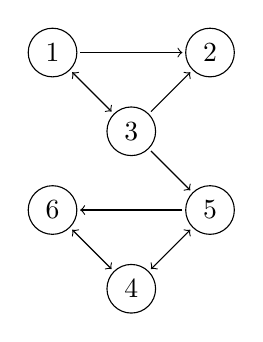
\begin{tikzpicture}
            \draw (0,0) node[circle,draw]{3};
            \draw (-1,1) node[circle,draw]{1};
            \draw (1,1) node[circle,draw]{2};
            \draw (-1,-1) node[circle,draw]{6};
            \draw (1,-1) node[circle,draw]{5};
            \draw (0,-2) node[circle,draw]{4};
        %
            \draw[<->] (-0.25,0.25) -- (-0.75,0.75);
            \draw[->] (-0.65,1) -- (0.65,1);
            \draw[->] (0.25,0.25) -- (0.75,0.75);
            \draw[->] (0.25,-0.25) -- (0.75,-0.75);
            \draw[->] (0.65,-1) -- (-0.65,-1);
            \draw[<->] (-0.75,-1.25) -- (-.25,-1.75);
            \draw[<->] (0.75,-1.25) -- (0.25,-1.75);
        \end{tikzpicture}
    \end{center}
        \caption{Sample graph of a web with six pages.}
        \label{fig:example_graph}
\end{figure}

We will first define some notation in the PageRank algorithm:
\begin{itemize}
    \item $|P_i|$ is the number of outlinks from page $P_i$
    \item $H$ is the {\it hyperlink} matrix defined as 
        \[ H_{ij} = \left\{ \begin{array}{cl} \frac{1}{|P_j|}, & \text{if there is a link
            from node $j$ to node $i$} \\ 0, & \text{otherwise} \end{array} \right. \]
        where the ``$i$'' and ``$j$'' are the row and column indices respectively.  
    \item $\bx$ is a vector that contains all of the PageRanks for the individual pages.
\end{itemize}

The PageRank algorithm works as follows:
\begin{enumerate}
    \item Initialize the page ranks to all be equal. This means that our initial
        assumption is that all pages are of equal rank.  In the case of Figure
        \ref{fig:example_graph} we would take $\bx_0$ to be 
        \[ \bx_0 = \begin{pmatrix} 1/6 \\ 1/6 \\ 1/6 \\ 1/6 \\ 1/6 \\ 1/6 \end{pmatrix}. \]
    \item Build the hyperlink matrix.  \\ As an example we'll consider node 3 in Figure
        \ref{fig:example_graph}.  There are three outlinks from node 3 (to nodes 1, 2, and
        5).  Hence $H_{13}=1/3$, $H_{23} = 1/3$, and $H_{53} = 1/3$ and the partially
        complete hyperlink matrix is
        \[ H = \begin{pmatrix} 
                - & - & 1/3 & - & - & - \\
                - & - & 1/3 & - & - & - \\
                - & - & 0   & - & - & - \\
                - & - & 0   & - & - & - \\
                - & - & 1/3 & - & - & - \\
                - & - & 0   & - & - & - 
            \end{pmatrix} \]
    \item The difference equation $\bx_{n+1} = H \bx_n$ is used to iteratively refine the
        estimates of the page ranks.  You can view the iterations as a person visiting a
        page and then following a link at random, then following a random link on the next
        page, and the next, and the next, etc.  Hence we see
        that the iterations evolve exactly as expected for a difference equation.
        \begin{center}
            \begin{tabular}{|c|c|}
                \hline
                Iteration & New Page Rank Estimation \\ \hline \hline
                0 & $\bx_0$ \\
                1 & $\bx_1 = H \bx_0$ \\
                2 & $\bx_2 = H \bx_1 = H^2 \bx_0$ \\
                3 & $\bx_3 = H \bx_2 = H^3 \bx_0$ \\
                4 & $\bx_4 = H \bx_3 = H^4 \bx_0$ \\
                \vdots & \qquad \vdots \\
                $k$ & $\bx_k = H^k \bx_0$ \\ \hline
            \end{tabular}
        \end{center}
    \item When a steady state is reached we sort the resulting vector $\bx_k$ to give the
        page rank. The node (web page) with the highest rank will be the top search
        result, the second highest rank will be the second search result, and so on.
\end{enumerate}

It doesn't take much to see that this process can be very time consuming.  Think about
your typical web search with hundreds of thousands of hits; that makes a square matrix $H$
that has a size of hundreds of thousands of entries by hundreds of thousands of entries!
The matrix multiplications alone would take many minutes (or possibly many hours) for
every search! \dots but Brin and Page were pretty smart dudes!!


We now state a few theorems and definitions that will help us simplify the iterative
PageRank process.
\begin{thm}\label{thm:eigen_expand}
    If $A$ is an $n \times n$ matrix with $n$ linearly independent eigenvectors $\bv_1,
    \bv_2, \bv_3,$ $\ldots, \bv_n$ and associated eigenvalues $\lambda_1, \lambda_2,
    \lambda_3, \ldots, \lambda_n$ then for any initial vector $\bx \in \mathbb{R}^n$ we
    can write $A^k \bx$ as
    \[ A^k \bx = c_1 \lambda_1^k \bv_1 + c_2 \lambda_2^k \bv_2 + c_3 \lambda_3^k \bv_3 +
        \cdots c_n \lambda_n^k \bv_n \]
    where $c_1, c_2, c_3, \ldots, c_n$ are the constants found by expressing $\bx$ as a
    linear combination of the eigenvectors. \\Note: We can assume that the eigenvalues are ordered
    such that $\lambda_1 \ge \lambda_2 \ge \lambda_3 \ge \cdots \ge \lambda_n$.
\end{thm}
\begin{proof}
    (Prove the preceding theorem)
\end{proof}

\begin{definition}
    A {\bf probability vector} is a vector with entries on the interval $[0,1]$ that add up to 1. 
\end{definition}
\begin{definition}
    A {\bf stochastic matrix} is a square matrix whose columns are probability vectors.
\end{definition}

\begin{thm} \label{thm:largest_ev_stochastic}
    If $A$ is a stochastic $n \times n$ matrix then $A$ will have $n$ linearly independent
    eigenvectors.  Furthermore, the largest eigenvalue of a stochastic matrix will
    \underline{always} be $\lambda_1 = 1$ and the smallest eigenvalue  will always be
    nonnegative: $0 \le \lambda_n < 1$.
\end{thm}

Some of the following tasks will ask you to {\it prove} a statement or a theorem.  This
means to clearly write all of the logical and mathematical reasons why the statement is
true. Your proof should be absolutely crystal clear to anyone with a similar mathematical
background \dots if you are in doubt then have a peer from a different group read your
proof to you \underline{out loud}.

\begin{problem}
    Finish writing the hyperlink matrix $H$ from Figure \ref{fig:example_graph}.
\end{problem}

\begin{problem}
    Write MATLAB code to implement the iterative process defined previously. Make a plot
    that shows how the rank evolves over the iterations.
\end{problem}


\begin{problem}
    What must be true about a collection of $n$ pages such that an $n\times n$
        hyperlink matrix $H$ is a stochastic matrix.
\end{problem}

The statement of the next theorem is incomplete, but the proof is given to you.  Fill in
the blank in the statement of the theorem and provide a few sentences supporting your
answer.
\begin{thm}\label{thm:steady}
    If $A$ is an $n \times n$ stochastic matrix and $\bx_0$ is some initial vector
    for the difference equation $\bx_{n+1} = A \bx_n$, then the steady state
    vector is
    \[ \bx_{equilib} = \lim_{k \to\infty} A^k \bx_0 = \underline{\hspace{1in}}. \]
\end{thm}
\begin{proof}
    First note that $A$ is an $n \times n$ stochastic matrix so from Theorem
    \ref{thm:largest_ev_stochastic} we know that there are $n$ linearly
    independent eigenvectors.  We can then substitute
    the eigenvalues from Theorem \ref{thm:largest_ev_stochastic} in Theorem
    \ref{thm:eigen_expand}. Noting that if $0<\lambda_j<1$ we have $\lim_{k \to
    \infty} \lambda_j^k = 0$ the result follows immediately.
\end{proof}
\begin{problem}
    Discuss how Theorem \ref{thm:steady} greatly simplifies the PageRank iterative process
    described previously.  In other words: there is no reason to iterate at all.  Instead,
    just find \underline{\hspace{1in}}.
\end{problem}
\begin{problem}
\item Now use the previous two problems to find the resulting PageRank vector from the web in Figure
    \ref{fig:example_graph}?  Be sure to rank the pages in order of importance.
    Compare your answer to the one that you got in problem 2.
\end{problem}


\begin{problem}
    Consider the web in Figure \ref{fig:graph2}.
        \begin{enumerate}
            \item[(a)] Write the $H$ matrix and find the initial state $\bx_0$, 
            \item[(b)] Find
                steady state PageRank vector using the two different methods described:
                one using the iterative difference equation and the other using Theorem
                \ref{thm:steady} and the dominant eigenvector.
            \item[(c)] Rank the pages in order of importance.
        \end{enumerate}
\end{problem}
\begin{figure}[ht!]
    \begin{center}
        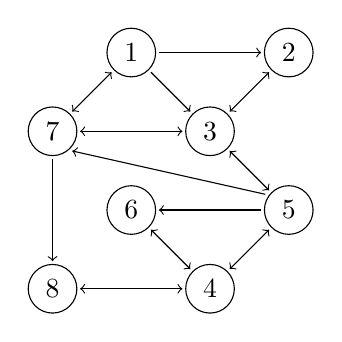
\begin{tikzpicture}
            \draw (0,0) node[circle,draw]{3};
            \draw (-1,1) node[circle,draw]{1};
            \draw (1,1) node[circle,draw]{2};
            \draw (-1,-1) node[circle,draw]{6};
            \draw (1,-1) node[circle,draw]{5};
            \draw (0,-2) node[circle,draw]{4};
            \draw (-2,0) node[circle,draw]{7};
            \draw (-2,-2) node[circle,draw]{8};
        %
            \draw[<-] (-0.25,0.25) -- (-0.75,0.75);
            \draw[->] (-0.65,1) -- (0.65,1);
            \draw[<->] (0.25,0.25) -- (0.75,0.75);
            \draw[<->] (0.25,-0.25) -- (0.75,-0.75);
            \draw[->] (0.65,-1) -- (-0.65,-1);
            \draw[<->] (-0.75,-1.25) -- (-.25,-1.75);
            \draw[<->] (0.75,-1.25) -- (0.25,-1.75);
            \draw[<->] (-1.75,0.25) -- (-1.25,0.75);
            \draw[<->] (-1.65,0) -- (-0.35,0);
            \draw[<-] (-1.75,-0.25) -- (0.7,-0.8);
            \draw[->] (-2,-0.35) -- (-2,-1.65);
            \draw[<->] (-1.65,-2) -- (-0.35,-2);
        \end{tikzpicture}
    \end{center}
    \caption{Graph of a web with eight pages.}
    \label{fig:graph2}
\end{figure}


\begin{problem}
    One thing that we didn't consider in this version of the Google Page Rank algorithm is
    the random behavior of humans.  One, admittedly slightly naive, modification that we
    can make to the present algorithm is to assume that the person surfing the web will
    randomly jump to any other page in the web at any time.  For example, if someone is on
    page 1 in Figure \ref{fig:graph2} then they could randomly jump to any page 2 - 8.
    They also have links to pages 2, 3, and 7.  That is a total of 10 possible next steps
    for the web surfer.  There is a $2/10$ chance of heading to page 2.  One of those is
    following the link from page 1 to page 2 and the other is a random jump to page 2
    without following the link.  Similarly, there is a $2/10$ chance of
    heading to page 3, $2/10$ chance of heading to page 7, and a $1/10$ chance of randomly
    heading to any other page.

    Implement this new algorithm, called the {\it random surfer algorithm}, on the web in
    Figure \ref{fig:graph2}.  Compare your ranking to the non-random surfer results from
    the previous problem.
\end{problem}



% \section{Principal Component Analysis (Incomplete)}


\section{Exercises}

\begin{problem}
    Write code to solve the following systems of equations via both LU and QR
    decompositions.
    \begin{enumerate}
        \item[(a)] 
            \[ \begin{array}{rl} x + 2y + 3z &= 4 \\ 2x + 4y + 3z &= 5 \\ x + y &= 4
                \end{array} \]
        \item[(b)] 
            \[ \begin{array}{rl} 2y + 3z &= 4 \\ 2x + 3z &= 5 \\ y &= 4
                \end{array} \]
        \item[(b)] 
            \[ \begin{array}{rl} 2y + 3z &= 4 \\ 2x + 4y + 3z &= 5 \\ x+y &= 4
                \end{array} \]
    \end{enumerate}
\end{problem}
\hint{
    Remember that if $A \bx = \bb$ and $A$ is square then we first factor $A = LU$ and the
    system becomes $LU \bx = \bb$.  Defining $\by = U \bx$ we solve $L \by = \bb$ with a
    lower triangular solve and then
    solve $U \bx = \by$ with an upper triangular solve.

    If we use the QR factorization then $A = QR$ and the system becomes $QR\bx = \bb$.
    Recalling that $Q$ is an orthonormal matrix we only need to solve $R \bx = Q^T \bb$
    with an upper triangular solve.
}


\begin{problem}
    In this exercise we will use numerical linear algebra to do some handwriting
    recognition on the classical data set \mcode{mnist}.  The \mcode{mnist} data set
    contains a training set of 60,000 numbers and a test set of 10,000 numbers.  Each
    digit in the database was placed in a 28 by 29 grayscale image such that the center of
    mass of its pixels is at the center of the picture.  While our primary goal for this
    problem is to use numerical linear algebra, our secondary goal is to get some
    experience with the logic of machine learning.  In machine learning problems we often
    follow the following logic:
    \begin{itemize}
        \item First use a set of data for which we know the {\it answer} (in this case the
            {\it answer} is the numerical value of the digit that was written).  We call
            this the training data set in the sense that we train the numerical method
            with the correct answers in mind.
        \item Next we compare data with hidden answers to our training set and build a
            method for using the training set to make a prediction for the answer.  This
            is called the testing phase of a machine learning algorithm.  In the testing
            phase we know the {\it answer} but keep it hidden from the algorithm.  We let
            our algorithm predict the {\it answer} and then compare to the hidden truth.
            At the end of this step we can give a percent effectiveness for our algorithm.
        \item In the final step of a machine learning process we give the numerical
            algorithm data where we don't know the {\it answer} and use the algorithm to
            predict for us.  
    \end{itemize}

    Let's be more specific.  Let's say that we want to determine if a handwritten digit is
    the number ``0''.  From the training set we average all of the zeros together to get a
    best estimate of what a ``0'' looks like.  Then we build a mathematical technique for
    doing the comparison between our new digit and the averaged training 0.  If the
    comparison technique tells us that our new digit is {\it close enough} then we call
    that new digit a zero. We can do this for all of the \mcode{test} 0's and determine
    the percent effectiveness for our comparison technique. 

    {\bf Your Tasks:}
    \begin{enumerate}
        \item[(a)] Start by going to
            \href{http://www.cs.nyu.edu/~roweis/data.html}{www.cs.nyu.edu/$\sim$roweis/data.html}
            to download the data set.  Download the file titled \mcode{mnist_all.mat}.
            This file is a MATLAB file that needs to be read into your working session of
            MATLAB.  
        \item[(b)] To read the \mcode{mnist_all.mat} data into MATLAB \\
            \mcode{load mnist_all.mat}\\
            Then type \mcode{whos} to see the variables containing training digits
            (\texttt{train0, ..., train9}) and test digits (\texttt{test0, ...,
            test9}).
        \item[(c)] To visualize the first image in the matrix \texttt{train0} use 
\begin{lstlisting}
digit = train0(1,:); % read the first row all columns out of train0
digitImage = reshape(digit,28,28); % turn into a 28x28 matrix
image(rot90(flipup(digitImage),-1))
colormap(gray(256))
axis square tight off
\end{lstlisting}
        \item[(d)] Create a 10 by 784 matrix $T$ whose $i^{th}$ row contains the average
            pixel values over all of the training images of the number $i-1$.  For
            instance, the first row of $T$ can be formed by typing \\
            \mcode{T(1,:) = mean(train0);} \\
            Visualize these average digits using the \mcode{subplot} command creating a
            $2 \times 5$ matrix of plots with the average 0 in the upper left and the
            average 9 in the lower right.  Check yourself by making sure that your image
            is identical to Figure \ref{fig:mnist_average}.
        \item[(e)] We are going to try two methods for handwriting recognition.  There are
            10,000 test numbers that are not in the training set and we want to try two
            different ways of determining which digit is in the test image.  Your job is
            to implement both of these methods.  You need to test all 10,000 test images and
            gather statistics on how often the method identifies the test image.  Report
            your answers by stating the proportion of correct identifications for each of
            the 10 numerals.
            \begin{description}
                \item[Method \#1 (Min Norm):] Compare pixels in the test digit to each row of the
                    training matrix $T$ and determine which row most closely resembles the
                    test digit.  Pseudo code for this method is:
                    \begin{itemize}
                        \item Let $D$ be the first test digit in \texttt{test0} using \\
                            \mcode{D = double(test0(1,:));}
                        \item For each row $i=1, 2, \cdots, 10$ compute \\
                            \mcode{norm(T(i,:) - D)} \\
                            and determine which value of $i$ this is smallest
                        \item $D$ is probably the digit $i-1$.
                        \item repeat for all of the test digits in \texttt{test0},
                            \texttt{test1}, \ldots.
                    \end{itemize}
                    Be sure to write code to test all of the 10,000 test digits.  There
                    are elegant ways to code this but you can also complete this task with
                    a bunch of copy and paste.
                \item[Method \#2 (Min Projections):] Project the test image vector $D$
                    onto the mean training image $T(i,:)$ and find the error in the
                    projection.  In this method we seek to minimize the size of the error.
                    Recall that the projection of $D$ onto $T(i,:)$ is 
                    \[ \frac{D \cdot T(i,:)}{T(i,:) \cdot T(i,:)} \]
                    and the error in the projection is 
                    \[ \left\| D - \left( \frac{D \cdot T(i,:)}{T(i,:) \cdot T(i,:)} \right)
                    T(i,:) \right\| \]
            \end{description}
    \end{enumerate}
\end{problem}

\begin{figure}
    \begin{center}
        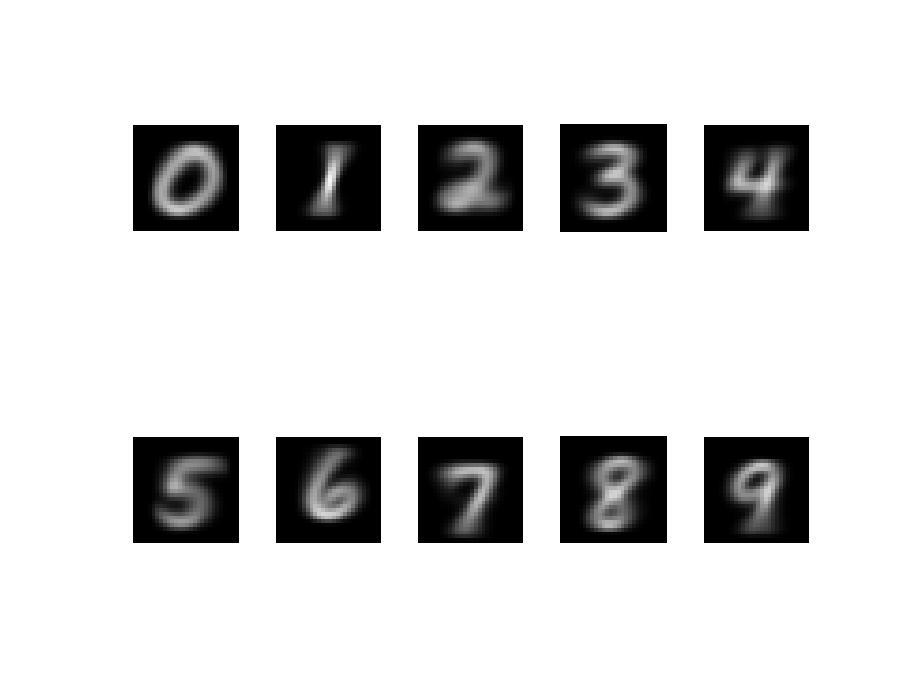
\includegraphics[width=0.9\columnwidth]{mnist_average_training_image.eps}
    \end{center}
    \caption{The 10 images are the averages of all of the training images for each digit.
        They represent what a {\it typical} digit should look like for each of the 10
    digits.}
    \label{fig:mnist_average}
\end{figure}



\begin{problem}
    Find a least squares solution to the equation $A \bx = \bb$ in two different ways with 
    \[ A = \begin{pmatrix} 1 & 3 & 5 \\ 4 & -2 & 6 \\ 4 & 7 & 8 \\ 3 & 7 & 19
        \end{pmatrix} \quad \text{and} \quad \bb = \begin{pmatrix} 5 \\ 2 \\ -2 \\
        8\end{pmatrix}. \]
\end{problem}
\hint{
    This is a rectangular system so be careful with your implementation of algorithms.
    You can't do an LU factorization directly on $A$.
}

\begin{problem}
    Find the largest eigenvalue of the matrix $A$ WITHOUT using the built in
    ``\mcode{eig}'' or ``\mcode{eigs}'' commands in MATLAB.
    \[ A = \begin{pmatrix} 1 & 2 & 3 & 4 \\ 5 & 6 & 7 & 8 \\ 9 & 0 & 1 & 2 \\ 3 & 4 & 5 &
        6 \end{pmatrix} \]
\end{problem}
\hint{
    You should be using the power method.
}


\begin{problem}
    Find a least square cubic function that best fits the following data. Solve this
    problem with Excel and with MATLAB using the normal equations.
    \begin{center}
        \begin{tabular}{|c|c|}
            \hline
            $x$ & $y$ \\\hline \hline
            0   & 1.0220\\
            0.0500&   1.0174\\
            0.1000&   1.0428\\
            0.1500&   1.0690\\
            0.2000&   1.0505\\
            0.2500&   1.0631\\
            0.3000&   1.0458\\
            0.3500&   1.0513\\
            0.4000&   1.0199\\
            0.4500&   1.0180\\
            0.5000&   1.0156\\
            0.5500&   0.9817\\
            0.6000&   0.9652\\
            0.6500&   0.9429\\
            0.7000&   0.9393\\
            0.7500&   0.9266\\
            0.8000&   0.8959\\
            0.8500&   0.9014\\
            0.9000&   0.8990\\
            0.9500&   0.9038\\
            1.0000&   0.8989 \\\hline
        \end{tabular}
    \end{center}
\end{problem}


\begin{problem}
    The following iterative sequence is defined for the set of
    positive integers:
    \begin{flalign*}
        & n \to \frac{n}{2} \quad \text{(n is even)} \\
        & n \to 3n + 1 \quad \text{(n is odd)}
    \end{flalign*}
    Using the rule above and starting with $13$, we generate the following sequence:
    \[ 13 \to  40 \to 20 \to 10 \to 5 \to 16 \to 8 \to 4 \to 2 \to 1 \]
    It can be seen that this sequence (starting at 13 and finishing at 1) contains 10
    terms. Although it has not been proved yet (Collatz Problem), it is thought that all
    starting numbers finish at 1.

    Write code to determine which starting number, under one million, produces the longest
    chain? NOTE: Once the chain starts the terms are allowed to go above one million
\end{problem}
% \solution{Source: Project Euler Problem \#14: Solution: 837799}


\begin{thm}[Eigen-Structure of Symmetric Matrices]\label{thm:symmetric_matrix_thm}
    If $A$ is a symmetric matrix with eigenvalues $\lambda_1, \lambda_2, \ldots,
    \lambda_n$ then $|\lambda_1| > |\lambda_2| > \cdots > |\lambda_n|$.  Furthermore, the
    eigenvectors will be orthogonal to each other. 
\end{thm}


\begin{problem}
    For symmetric matrices we can build an extension to the Power Method in order
    to find the second most dominant eigen-pair for a matrix $A$.  Theorem
    \ref{thm:symmetric_matrix_thm} suggests the following method for finding the second
    dominant eigen-pair for a symmetric matrix.  This method is called the {\bf deflation
    method}.
    \begin{itemize}
        \item Use the power method to find the dominant eigenvalue and eigenvector.
        \item Start with a random unit vector of the correct shape.
        \item Multiplying your vector by $A$ will {\it pull it toward} the dominant
            eigenvector.  After you multiply, project your vector onto the dominant
            eigenvector and find the projection error.  
        \item Use the projection error as the new approximation for the eigenvector.
    \end{itemize}    

    Note that the deflation method is really exactly the same as the power method with the
    exception that we orthogonalize at every step.  Hence, when you write your code expect
    to only change a few lines from your Power method.

    Write a
    MATLAB function \mcode{MyPower2} to find the second largest eigenvalue and
    eigenvector pair by putting the deflation method into practice. Test your code on a
    \underline{symmetric} matrix $A$ and compare against MATLAB's \mcode{eig} command.
    Your code needs to work on symmetric matrices of arbitrary size and you need to write
    test code that clearly shows the error between your calculated eigenvalue and MATLAB's
    eigenvalue as well as your calculated eigenvector and MATLAB's eigenvector.\\ To
    guarantee that you start with a symmetric matrix you can use the following code.
\begin{lstlisting}
N = 40; % size of the matrix ... make this large-ish
A = rand(N,N);
A = A'*A; % this will be a random symmetric NxN matrix.
\end{lstlisting}
\end{problem}
\hint{
    Technically speaking you don't have to orthogonalize at every step so if you want to
    make your code more efficient you can orthogonalize every $k^{th}$ step (for your
    choice of $k$).  It would be cool to check what this does to the efficiency of your
    algorithm.
}
